\documentclass[sigplan,10pt,nonacm]{acmart}
\settopmatter{printfolios}

\makeatletter
\def\ps@headings{%
\def\@oddhead{\mbox{}\scriptsize\rightmark \hfil \thepage}%
\def\@evenhead{\scriptsize\thepage \hfil \leftmark\mbox{}}%
\def\@oddfoot{}%
\def\@evenfoot{}}
\makeatother
\raggedbottom
\graphicspath{ {./graphs/} }

\pagestyle{plain}
\settopmatter{printfolios=true}

%\usepackage[small,compact]{titlesec}
\usepackage{epsfig}
\usepackage{graphicx}
\usepackage{xspace}
\usepackage{listings}
\usepackage{multirow}
\usepackage{listings}
\usepackage{color}
\usepackage{caption}
\usepackage{subcaption}
\usepackage[ruled,vlined]{algorithm2e}
\usepackage{algorithmic}
\usepackage{amsmath}
\usepackage{tikz}
\usepackage{pgfplots}
\usepackage{multicol}
\pgfplotsset{compat=1.12}
\newcounter{algorithm}


\definecolor{mygreen}{rgb}{0,0.6,0}
\definecolor{mygray}{rgb}{0.5,0.5,0.5}
\definecolor{mymauve}{rgb}{0.58,0,0.82}

\lstset{ 
  backgroundcolor=\color{white},   % choose the background color; you must add \usepackage{color} or \usepackage{xcolor}; should come as last argument
  basicstyle=\footnotesize,        % the size of the fonts that are used for the code
  breakatwhitespace=false,         % sets if automatic breaks should only happen at whitespace
  breaklines=true,                 % sets automatic line breaking
  captionpos=b,                    % sets the caption-position to bottom
  commentstyle=\color{mygreen},    % comment style
  deletekeywords={...},            % if you want to delete keywords from the given language
  escapeinside={\%*}{*)},          % if you want to add LaTeX within your code
  extendedchars=true,              % lets you use non-ASCII characters; for 8-bits encodings only, does not work with UTF-8
  %firstnumber=1000,                % start line enumeration with line 1000
  frame=single,	                   % adds a frame around the code
  keepspaces=true,                 % keeps spaces in text, useful for keeping indentation of code (possibly needs columns=flexible)
  keywordstyle=\color{blue},       % keyword style
  language=C,                 % the language of the code
  morekeywords={*,...},            % if you want to add more keywords to the set
  numbers=none,                    % where to put the line-numbers; possible values are (none, left, right)
  numbersep=5pt,                   % how far the line-numbers are from the code
  numberstyle=\tiny\color{black}, % the style that is used for the line-numbers
  rulecolor=\color{black},         % if not set, the frame-color may be changed on line-breaks within not-black text (e.g. comments (green here))
  showspaces=false,                % show spaces everywhere adding particular underscores; it overrides 'showstringspaces'
  showstringspaces=false,          % underline spaces within strings only
  showtabs=false,                  % show tabs within strings adding particular underscores
  %stepnumber=2,                    % the step between two line-numbers. If it's 1, each line will be numbered
  stringstyle=\color{mymauve},     % string literal style
  tabsize=2,	                   % sets default tabsize to 2 spaces
  title=\lstname                   % show the filename of files included with \lstinputlisting; also try caption instead of title
}

\usepackage{url}
%\usepackage[hyphens]{url}
\usepackage{hyperref}
%\hypersetup{breaklinks=true}
%\usepackage[margin=10pt]{subcaption}
%\usepackage{subcaption}

% Other useful macros
\newcommand{\fixme}[1]{\textbf{FIX: #1}}
\newcommand{\codesm}[1]{\texttt{\small #1}}
\newcommand{\implication}{\vspace{0.1in} \noindent \emph{Implication:~}}
\newcommand{\fig}[4]{%
  \begin{figure}[ht]%
    %\frame{\includegraphics[#1]{#2}}
    \includegraphics[#1]{#2}
    \caption{{#3}}\label{#4}
\end{figure}
}

\newcommand{\question}[1]{\textbf{DOUBT: #1}}

\def \sec {\S}



\begin{document}
\widowpenalty=5000
\clubpenalty=5000


\title{\textsf{A Comparative Study on Dynamic Service Function Chaining in SDN-Enabled Networks}}


\author{ Srilakshmi Bharadwaj(smbharadwaj@wisc.edu), Sakshi Bansal(sakshi@cs.wisc.edu), Jatin Arora(jarora4@wisc.edu)}


\begin{abstract}

In this paper, we do a comparative study of three different service function chaining algorithms. First Algorithm is Max Throughput Routing Algorithm \cite{ref:paper1} which is an offline algorithm. Second is an online algorithm based on Linear Programming, Primal Dual Update Algorithm \cite{ref:paper1}. Third is the RA-RA algorithm \cite{ref:paper2} which is also an online routing algorithm based on Binary Integer Programming. We experiment on two different topologies, Fat-Tree \cite{ref:fat-tree} from \cite{ref:paper1} and CORONET CONUS \cite{ref:coronus} from \cite{ref:paper2}. The results of the experiments are presented by plotting the achievable throughput against the number of flows. We are able to show that the offline Max Throughput Routing Algorithm outperforms both online algorithms. Also, among the two online algorithms we show that Primal Dual Update Algorithm performs better than the RA-RA algorithm. 


\end{abstract}


\maketitle


\section{Introduction}
\label{sec:intro}

Today, a humongous amount of data goes through various access networks, enterprise networks, data centers, cloud computing environments. These network systems require data to go through multiple network/service functions in a specific order. This gives rise to the notion of Service Function Chaining. On the other hand, many data centers have started adopting SDN based architecture. 

Being controlled by a centralized controller, SDNs open a completely new possibility of designing routing algorithms for service function chaining. There can be multiple deployments of a particular network function, hence there can be multiple paths chosen by a single flow depending upon the available resources. While directing traffic flow through these networks, we can maximize the throughput by choosing the optimal path while making sure that the service function chain requirement is satisfied. 

The complexity of this problem can be demonstrated with the network depicted in Figure~\ref{fig:nw_example}. This network contains four types of VNFs and each of them has multiple instances deployed. For example, VNF11, VNF12 and VNF13 indicate the first, second and third instances of VNF1 respectively. Now suppose that there's a flow with SFC request which starts from node A and has to traverse the instances of VNF1, VNF2, VNF3 and VNF4 before arriving at node J. As we can see in this network, there exists many paths (such as the dotted lines marked with different colors) that traverse different VNF instances and can satisfy the requirement. Therefore, the challenge for dynamic SFC formation is to make an optimal strategy selecting VNF instances from multi-instance NFV environment and routing flows with SFC requests to traverse these selected VNF instances in predefined orders.

\fig{width=\columnwidth}{VNF}{\textmd{A sample network with function nodes and service chaining specifications ~\cite{ref:paper2}}}{fig:nw_example}

This motivates us to study different traffic routing algorithms being proposed by various researchers, implement them and do a comparative study to determine the algorithm that works best in terms of throughput in various scenarios.

The traffic routing algorithms can broadly be divided into two classes - offline and online. In the case of offline routing algorithms it can be assumed that all required traffic demands are available a prior whereas in the case of online algorithms, the decisions have to be made using only the current state of network and the incoming flow. Since, the offline algorithms have more information about sets of network flows they generally result in a better network allocation. The downside however is that they take more time which can violate QoS requirements for flows and thus their use in real-time scenarios is limited.

In this paper we studied the offline algorithm Traffic-Merging Algorithm (TMA) proposed in ~\cite{ref:paper1}. We implemented TMA with goal of maximising throughput while putting constraints on link capacity, processing capacity usage of a middle box and number of routing rules installed for this flow. This utility problem as it turns out is NP hard. TMA, in the first phase, solves the optimization problem by formulating it as a constrained linear optimization problem and ignoring the non-convex constraint on number of rules that can be installed on a switch. TMA in the second phase then addresses the constraint on rules installed on switches by using a merge operator. This merge operator merges the routing rules obtained from the first phase and guarantees an upper bound on number of rules that need to be installed on switches without compromising on the network throughput. Since the merge operator does not change the network throughput obtained from linear optimization problem, as part of this paper, we only use the output from the first phase of this algorithm which we call Max Throughput Routing Algorithm or MTRA (the linear optimization problem) for our throughput calculation. 


For analysing algorithms in online environment, we compared Primal-Dual-Update Algorithm (PDA) proposed in ~\cite{ref:paper1} and RA-RA proposed in ~\cite{ref:paper2}. PDA accepts or rejects a new flow by keeping parsimonious price variables for each resource. PDA has a system parameter which allows a trade off in algorithm competitiveness in maximizing throughput and the routing scheme performance in meeting delay requirements. The values of this parameter is in the range of 0 to 1. This algorithm approaches offline optimum as this parameter approaches 0. RA-RA is a Differentiated Routing Problem considering SFC(DRP-SFC). It is formulated as a Binary Integer Programming(BIP) model. RA-RA solves DRP-SFC to obtain the routing that maximises the throughput of the network by ensuring efficient consumption of resources.


The rest of the paper is organised as follows: Section~\ref{sec:problemdef} gives an overview of problem formulation for the three algorithms in consideration, Section~\ref{sec:setup} talks about our experimental setup for the comparison of these algorithms and in Section~\ref{sec:results} we evaluate the results. We also discuss the related works in the field in Section~\ref{sec:relatedwork}. Finally, we conclude and discuss future work in Section~\ref{sec:conclusion}.



\section{Problem Formulation}
\label{sec:problemdef}

Software-defined networks (SDNs) are one of the emerging architectures in network design that can be programmed, made cost-efficient and are highly effective. As the SDNs are managed centrally using a controller,  many new algorithms have been proposed to improve the performance of networks with network functions. Our goal is to investigate the algorithms of maximizing throughput in SDN-enabled networks with dynamic service function chaining. Two types of algorithms are proposed in ~\cite{ref:paper1}  for two traffic routing scenarios: offline, where flows and their demands are known beforehand(Traffic Merging Algorithm TFA) and online where flows arrive one at a time and the routing decision is based on the current state of the network(Primal-Dual Update Algorithm PDA). In our project, we aim to present a comparative study of the above algorithms with the RA-RA algorithm proposed in ~\cite{ref:paper2}\\

\subsection{Max Throughput Routing and Primal Dual Update Algorithm \cite{ref:paper1}}
\subsubsection{System Model}
The network is modeled as a graph G := (V, E), where V is the set of vertices and E is the set of edges. Every edge e $\in$ E is associated with a capacity C(e). Every vertex m $in$ V on which a middlebox is deployed is associated with a processing capacity P(m). The set of middlebox types is represented as M. Every flow l is characterised by a source node s, destination node t and the set of middlebox types(Service Function Chain or SFC) it needs to traverse. This is represented as : \newline
$$R(l) = {(s, m_1, m_2, t)} : m_1 \in M_1, m_2 \in M_2$$\\
From R(l), the set of paths between a given source and destination and traversing the required chain of middlebox types, is computed, using the shortest path algorithm(BFS). Multiple instances of each middlebox type can be deployed at different nodes in the network. Each path in the set of admissible paths $r \in  R(l)$, is associated with usage of link e by $G_r(e)$ and usage of processing capacity at a middlebox m by $Q_r(m)$.
\newline

\subsubsection{Max Throughput Routing Algorithm (MTRA) - Offline}
Here we assume the set of flows L is given. This information can be collected by SDN switches and is used in applications where bandwidth is allocated based on predefined service-level agreement.

For every admissible path $r \in R(l)$, for a given flow l, we determine a splitting portion $x_{rl}$. This splitting would occur at the IP flow level and not at the packet level as indicated in \cite{ref:paper1}. The splitting portion is determined by solving a linear programming model referred to as the Global-OPT. The objective of Global-OPT is to achieve global routing optimization by determining the best route that a given flow l can be routed through. In determining the best route for a given set of flows, the goal would be to maximize the overall throughput while satisfying the constraints (1), (2), (3) and (4) and shown in Algorithm 1. Constraint (1) represents flow splitting, (2) ensures that the load on a particular edge while routing a flow along r does not exceed the capacity of the, (3) ensures that the middlebox processing power consumption is within its capacity and (4) is the positivity constraint.

\subsubsection{Primal Dual Update Algorithm (PDA) - Online}
The set of flows L is not given. Flows are served one at a time. Every resource is associated with a "shadow price" as indicated in \cite{ref:paper1}. When there is an incoming flow, shadow price is computed and compared to a present threshold. Based on the comparison, the flow is accepted or rejected. If accepted, the shadow price is updated to reflect the resource consumption of that particular flow. This is shown in Algorithm 2. 

Every admissible path r is associated with a path price,\\
$$K_r := \sum_{e}G_r(e)\lambda(e) + \sum_{m}Q_r(m)\theta(m)$$\\
The constant $B^*$ indicates the maximum usage of each resource over all possible paths for the flows:

$$B^* = \max_{l,r}\{\max_{e}G_r(e), \max_{m}Q_r(m)\}$$

This constant controls the cost of the flow. $\epsilon$ can be set to a value in (0,1). It provides a tradeoff between the maximizing the network throughput and satisfying all the flow constraints. It is observed that when $\epsilon = 0$, the online algorithm(PDA) provides the same throughput as the offline case(MTRA). 

\begin{algorithm}
\SetAlgoLined
Solve Global-OPT with constraints (1), (2), (3), (4) \\
to get the routing X that maximizes the throughput \\
achieved \newline
Constraints:

\hspace{2mm}(1)\hspace{5mm}$\forall l : $\sum_{r\in R(l)}$ x_{rl} <= 1$

\hspace{2mm}(2)\hspace{5mm}$\forall e : $\sum_{l\in L}$ $\sum_{r\in R(l)}$ x_{rl}f_lG_r(e) <= C(e)$

\hspace{2mm}(3)\hspace{5mm}$\forall m : $\sum_{l\in L}$ $\sum_{r\in R(l)}$ x_{rl}f_lQ_r(m) <= P(m)$

\hspace{2mm}(4)\hspace{5mm}$\forall r,l : x_{rl} >= 0$

To maximize throughput: 

$$T : \sum_{l\in L} \sum_{r\in R(l)} x_{rl}f_l$$

\caption{Max-Throughput-Routing-Algorithm (MTRA)}
\end{algorithm}

\begin{algorithm}

$\chi \gets \frac{B^*}{\epsilon}$ \newline
\text{Initialize the dual variables to zero: }\newline
$\lambda(e) \gets 0 \hspace{2mm}\forall e$ \newline
$\theta(m) \gets 0 \hspace{2mm} \forall m$ \newline
$\pi(l) \gets 0 \hspace{2mm} \forall l$ \newline

\textbf{for} each arrival of flow request l \textbf{do} \newline
\hspace{5mm} $r^* \gets argmin_{r \in R(l)}K_r$ \newline
\hspace{10mm} \textbf{if} $K_{r^{*} \ge 1 \textbf{then}
} \ge 1$ \textbf{then} \newline
\hspace{15mm} Reject the request l and set $\pi(l) \gets 0$ \newline
\hspace{5mm} \textbf{else} \newline
\hspace{10mm} Route l through $r^*$ \newline
\hspace{10mm} $\pi(l) \gets f_l[1-K_{r^*}]$ \newline
\hspace{10mm} $\forall e $: \hspace{5mm} $\lambda(e) \gets \lambda(e)[1 + \frac{f_lG_{r^*}(e)}{C(e)}] + \frac{f_lG_{r^*}(e)}{\chi C(e)}$ \newline
\hspace{10mm} $\forall m$ : \hspace{5mm} $\theta(m) \gets \theta(m)[1 + \frac{f_lQ_{r^*}(m)}{P(e)}] + \frac{f_lQ_{r^*}(m)}{\chi P(m)}$
    
 \caption{Primal-Dual-Update-Algorithm (PDA)}
\end{algorithm}

\subsection{Resource Aware Routing Algorithm (RA-RA) \cite{ref:paper2}}
\subsubsection{System Model}
The network is represented as a graph G := (V, L), where V is the set of vertices and L is the set of links. M is the set of VNF types. Every node $u \in V$, on which an instance of VNF is deployed is associated with CPU capacity denoted as $C_u^{cpu}$. Every link $uv \in L$ is associated with a bandwidth capacity denoted by $C_{uv}^{bw}$. The $i^{th}$ flow's SFC request consists of a source node $S_i$, destination node $T_i$, the VNF chain that the flow has to traverse $\Omega_i$, bandwidth consumption $F_i^{bw}$ and CPU consumption $F_i^{cpu}$.\\
$$SFCR_i = \{S_i, T_i, \Omega_i, F_i^{bw}, F_i^{cpu}\}$$
$$\Omega_i = \{\Omega_i(1), \Omega_i(2), ..., \Omega_i(l)\}$$
Each j in $\Omega_i(j)$, represents a VNF type. While routing a flow i, $r_{i,u}^{cpu}$ represents the ratio of remaining CPU on node u and $r_{i,uv}^{bw}$ represents the ratio of remaining bandwidth on link uv. We will not be considering the flow table capacity($C_u^{ft}$) or consumption($r_u^{ft}$) in order to keep it consistent with MTRA and PDA.

\subsubsection{RA-RA algorithm}
The function Construct LFG($\hat{G}$) transforms the network graph into a Logical Function Graph(LFG) as shown in Function 1(Figure \ref{fig:lfg_construct}). LFG is a digraph which consists of source node, destination node and the set of VNF instances that is request by a particular flow. On arrival of a flow request i, we enumerate the set of VNF instances corresponding to a VNF type $\Omega_i(j)$, and list them in the same column. A link in LFG connects a node from previous column to all the nodes in the corresponding next column. This link is obtained by determining the shortest path between the pair of nodes from the original network graph. The cost of the link in LFG is the total relative costs of bandwidth and CPU consumed. The relative costs are inversely proportional to the remaining resources and are calculated as follows:\\
$$v_{i,\hat{u}\hat{v}} = \sum_{uv \in L} v_{i,uv}^{bw}z_{i,uv}^{\hat{u}\hat{v}} + \frac{v_{i,\pi(\hat{u})}^{cpu} + v_{i,\pi(\hat{v})}^{cpu}}{2}, \forall \hat{u}\hat{v} \in \hat{L}_i, \forall \hat{u}\hat{v} \in \hat{V}_i$$,
where, $v_{i,uv}^{bw}$ is the relative cost of bandwidth,  $v_{i,\pi(\hat{u})}^{cpu}$\ and $v_{i,\pi(\hat{v})}^{cpu}$ are the relative costs of CPU calculated as follows:\\
$$v_{i,uv}^{bw} = \frac{\max_{uv \in L}C_{uv}^{bw}}{r_{i,uv}^{bw}C_{uv}^{bw} - F_i^{bw}}$$
$$v_{i,u}^{cpu} = \frac{\max_{u \in V}C_{u}^{cpu}}{r_{i,u}^{cpu}C_{u}^{cpu} - F_i^{cpu}}$$
$\pi(.)$ is used to obtain the node on which a particular VNF instance is deployed. $z_{i,uv}^{\hat{u}\hat{v}} = 1$, if $\hat{u}\hat{v} \in \hat{L}_i$ traverses $uv \in L$ and $u \in V$. Here, $\hat{L}_i$ represents the set of links in the LFG and $\hat{V}_i$ represents the set of vertices in the LFG. An example of the LFG obtained from Function 1(Figure \ref{fig:lfg_construct}) is shown in Figure \ref{fig:lfg_solve}. In this example, the requested VNF types in $SFCR_i$ are 1,2,3 and 4. The VNF instances corresponding to each type is added in the same column. For example, VNF instances corresponding tu type 1(VNF11, VNF12 and VNF13) are added to the same column. A link is added from source $S_i$ to each of the type 1 VNF instances.

Once the LFG is constructed, we determine the shortest path satisfying the flow request i as shown in the RA-RA algorithm in Figure \ref{fig:RARA}. The cost of the path is the total relative cost of all the links in the path which is calculated as follows:\\
$$ \sum_{\bar{u}\bar{v} \in \bar{L}_i}\sum_{\hat{u}\hat{v} \in \hat{L}_i} v_{i, \hat{u}\hat{v}} z_{i,\hat{u}\hat{v}}^{\bar{u}\bar{v}}$$,
Here, $\bar{u}\bar{v} \in \bar{L}_i$ is the set of links in the Service Function Graph(SFG). SFG is obtained by concatenating the source node, VNF instance types and destination node in $SFCR_i$ in that order. $z_{i,\hat{u}\hat{v}}^{\bar{u}\bar{v}} = 1$, if $\bar{u}\bar{v} \in \bar{L}_i$ traverses $\hat{u}\hat{v} \in \hat{L}_i$.
The path computed should have minimum cost and satisfy the following constraints:\\
$$\sum_{\bar{u}\bar{v} \in \bar{L}_i} F_i^{bw} z_{i, uv}^{\bar{u},\bar{v}} \le r_{i,uv}^{bw}C_{uv}^{bw}, \forall uv \in L$$
$$\sum_{\bar{u} \in \bar{V}_i}\sum_{m \in M} F_i^{cpu}x_{i,m}^{\bar{u}}y_u^m \le r_{i,u}^{cpu}C_u^{cpu}, \forall u \in V$$
The above constraints ensure that the bandwidth and CPU consumption of a flow does not exceed the capacity of a particular link or a node respectively in the network. $z_{i, uv}^{\bar{u},\bar{v}} = 1$ if $\bar{u}\bar{v}$ traverses node u. $x_{i,m}^{\bar{u}} = 1$ if $\bar{u}$ is served by VNF instance m and $y_u^m = 1$ if VNF instance m is hosted on u. If a flow does not satisfy these constraints RA-RA computes the next best flow. This continues for a total of K iterations. If the optimal path is not found after K iterations, the flow is rejected.

In the LFG graph shown in Figure \ref{fig:lfg_solve}, if the shortest path obtained is $S_i \rightarrow VNF11 \rightarrow VNF21 \rightarrow VNF31 \rightarrow VNF41 \rightarrow T_i$, this path is checked for the above constraints. If the path satisfies the constraints, the flow is routed through the path and the resource costs are updated.

\fig{width=\columnwidth}{RA-RA-new}{\textmd{RA-RA Algorithm \cite{ref:paper2}}}{fig:RARA}
\fig{width=\columnwidth}{LFG}{\textmd{LFG Construction \cite{ref:paper2}}}{fig:lfg_construct}
\fig{width=\columnwidth}{LFG-solve}{\textmd{LFG obtained from Function 1 \cite{ref:paper2}}}{fig:lfg_solve}

\section{Experimental Setup}
\label{sec:setup}




\begin{figure*}
 
    \begin{multicols}{2}
    %\begin{minipage}
    %\resizebox{\columnwidth}{!}{
    \begin{subfigure}{0.45\textwidth}
    
\begin{tikzpicture}
\begin{axis}[
    xlabel={\textbf{Number of Flows}},
    ylabel={\textbf{Throughput}},
    xtick=data,
    legend pos=north west]
    \addplot[mark=diamond*,thick,red] coordinates {
        (100, 304.9)
(200, 548.197)
(300, 733.797)
(400, 911.396)
(500, 1011.883)
(600, 1122.26)
(700, 1190.12)
(800, 1285.59)
(900, 1345.2)
(1000, 1403.6)
} node[pos=0.7,below,anchor=west];
    
    \addplot[mark=x,mark options={solid},blue,thick,dashed] coordinates {
(100, 295.7)
(200, 490.9)
(300, 659.7)
(400, 790.689)
(500, 871.11)
(600, 961.77)
(700, 1023.12)
(800, 1109.215)
(900, 1165.7)
(1000, 1211.51)
}node[pos=0.7,above,anchor=east];


    \addplot[mark=o,mark options={solid},green,thick, dashed] coordinates {
(100, 304.9)
(200, 581.4)
(300, 717.19)
(400, 756.8)
(500, 765.1)
(600, 765.1)
(700, 798.8)
(800, 794.2)
(900, 776.4)
(1000, 787.75)
}node[pos=0.7,above,anchor=east];


    \addplot[mark=o,mark options={solid},black,thick,dashed] coordinates {
(100, 304.9)
(200, 588.2)
(300, 892.38)
(400, 1182.7)
(500, 1498.9)
(600, 1813.26)
(700, 2109.3)
(800, 2420.2)
(900, 2742.2)
(1000, 3056.5)
}node[pos=0.7,above,anchor=east];



\legend{PDA($\epsilon$=0.5),PDA($\epsilon$=0.75), RA-RA, Upper Bound}
\end{axis}
\end{tikzpicture}
\caption{Throughput for Fat-Tree topology}
\label{fig:sub1}
 \end{subfigure}\hspace{8mm}
% \end{minipage}

% \begin{minipage}
    \begin{subfigure}{0.45\textwidth}
    \begin{tikzpicture}
    \begin{axis}[
        xlabel={\textbf{Number of Flows}},
    ylabel={\textbf{Throughput}},
    xtick=data,
    legend pos=north west]
        \addplot[mark=o,mark options={solid},blue,thick,dashed] coordinates {
        (50, 145.191)
(100, 304.9)
(200, 588.297)
(300, 764.896)

}node[pos=0.7,above,anchor=east];
    
            \addplot[mark=o,mark options={solid},black,thick,dashed] coordinates {
        (50, 145.191)
(100, 304.9)
(200, 588.297)
(300, 892.38)

}node[pos=0.7,above,anchor=east];

    
    \legend{TMA, Upper Bound}
\end{axis}
\end{tikzpicture}
\caption{Throughput for TMA in Fat Tree Topology}
\label{fig:sub2}
    \end{subfigure}
    \end{multicols}
    
%%%%%%%%%%%%%%%%%%%%%%%%CORONA TOPOLOGY%%%%%%%%%%%%%%%%%%%%%%%%%%
    \begin{multicols}{2}
    \begin{subfigure}{0.45\textwidth}
    
\begin{tikzpicture}
\begin{axis}[
    xlabel={\textbf{Number of Flows}},
    ylabel={\textbf{Throughput}},
    xtick=data,
    legend pos=north west]
    \addplot[mark=diamond*,thick,red] coordinates {
    
    (100, 304.95) 
(200, 588.29)
(300, 883.89)
(400, 1136.62)
(500, 1347.71)
(600, 1540.79)
(700, 1721.76 )
(800, 1863.39)
(900, 1994.049)
(1000, 2107.62 )

} node[pos=0.7,below,anchor=west];
    
    \addplot[mark=x,mark options={solid},blue,thick,dashed] coordinates {
(100, 304.950)
(200, 588.297)
(300, 852.097)
(400, 1036.900)
(500, 1176.405)
(600,1378.411006353427)
(700, 1522.9892794267275)
(800, 1620.582731192362)
(900, 1706.6110469952177)
(1000, 1797.9923385972693 )
}node[pos=0.7,above,anchor=east];


    \addplot[mark=o,mark options={solid},green,thick, dashed] coordinates {
(100,304.95008052735665)
(200,588.2975326187434)
(300,892.3815061809704)
(400,1089.2800311383057)
(500,1149.5154241140162)
(600,1154.9944623727408)
(700,1213.2833337717482)
(800,1213.7767212368615)
(900,1255.5802839175446)
(1000,1292.8601849607876)

}node[pos=0.7,above,anchor=east];


    \addplot[mark=o,mark options={solid},black,thick,dashed] coordinates {
(100,304.95008052735665)
(200,588.2975326187434)
(300,892.3815061809704)
(400,1182.7698631944063)
(500,1498.9758816081755)
(600,1813.2640738634966)
(700, 2109.33)
(800, 2420.242917993053)
(900,2742.263537968908)
(1000,3056.548111449543)

}node[pos=0.7,above,anchor=east];



\legend{PDA($\epsilon$=0.5),PDA($\epsilon$=0.75), RA-RA, Upper Bound}
\end{axis}
\end{tikzpicture}
\caption{Throughput for CORONET CONUS Topology}
\label{fig:sub3}
 \end{subfigure}\hspace{8mm}
% \end{minipage}

% \begin{minipage}
    \begin{subfigure}{0.45\textwidth}
    \begin{tikzpicture}
    \begin{axis}[
        xlabel={\textbf{Number of Flows}},
    ylabel={\textbf{Throughput}},
    xtick=data,
    legend pos=north west]
        \addplot[mark=o,mark options={solid},blue,thick,dashed] coordinates {
(100, 304.950)
(200, 588.297)
(300, 892.381)
(400, 1182.769)


}node[pos=0.7,above,anchor=east];
    
            \addplot[mark=o,mark options={solid},black,thick,dashed] coordinates {
(100,304.95008052735665)
(200,588.2975326187434)
(300,892.3815061809704)
(400,1182.7698631944063)


}node[pos=0.7,above,anchor=east];

    
    \legend{TMA, Upper Bound}
\end{axis}
\end{tikzpicture}
\caption{Throughput for TMA in CORONET CONUS Topology}
\label{fig:sub4}
    \end{subfigure}
    
    \end{multicols}
    
    
    %\end{minipage}
    %}
    
\caption{Performance in terms of network throughput for TMA, PDA and RA-RA over different topologies.}

    \label{fig:graph}
\end{figure*}


In this section we explain the platform, topologies, configuration we used for our experiment. As we were not bench marking the time and resource utilization of the algorithms, we ran our experiments on CloudLab, Amazon Web Services and Local Desktop and collaborated the results. These experiments can be found in \cite{ref:gitimpl}.

\subsection{Platform}
We initially planned to implement our routing algorithms in NS3, OPNET or Java Network Simulator. This would have helped us see graphical simulation of the network. At the same time, we would have needed to setup the complete environment and team would have required to learn new technologies.  As we moved ahead with studying different algorithms, we realized that we do not need a graphical simulation of the network to benchmark throughput and it will be a waste of effort to invest time in learning network simulation languages like Tcl, ns2 etc.  The algorithms find path to route the flows using Dijkstra and breadth first search and satisfy the required constraints using linear programming. Between MATLAB and Python, Python seemed more intuitive because of the availability of wide community support, inbuilt libraries for solving linear programming and flexibility of the language. Solving all the constraints, we finalized \textbf{Python Language and Env} for implementing the algorithms and running the experiments. 

\subsection{Topologies}
Network topologies can have a substantial effect on 
performance of the algorithm or network topology plays an important role in choosing the correct algorithm for network routing. \cite{ref:paper1} solve PDA and TMA algorithms, perform experiment on FAT-Tree and GEANT Topology where as the RA-RA algorithm \cite{ref:paper2} uses to CORONET CONUS topology to perform the experiments. To have a fair comparison, we use the FAT-TREE topology from the work on PDA and TMA in \cite{ref:paper1}  and CORONET CONUS topology from RA-RA proposed in ~\cite{ref:paper2} to do the comparative study. 

\subsubsection{Fat-Tree}
The Fat-Tree topology  ~\cite{ref:fat-tree} is a tree branch topology with a core layer, aggregation layer, edge layer and hosts. For our experiment, we had 16 Core Switches, 32 Aggregation Switches, 32 Edge Switches and 128 hosts. There are 8 different types of Virtual functions deployed on 24 function nodes. The function nodes are deployed on switches as separate machines(not the node itself). Each type has 3 middle boxes deployed randomly on the nodes of the fat tree.  
The capacities(bandwidth) of link in the Fat-Tree are as follows: 

1. 200 units/link between core and aggregation layer.

2. 100 units/link between aggregation layer and edge layer.

3. 100 units/link between edge and host layer. 

Each middle box is connected to the switch using a link with capacity 200 units. The processing power of the middle boxes is limited to 300 units. 

\subsubsection{CORONET CONUS}
\begin{figure}[ht]
\vskip 0.2in
\begin{center}
\centerline{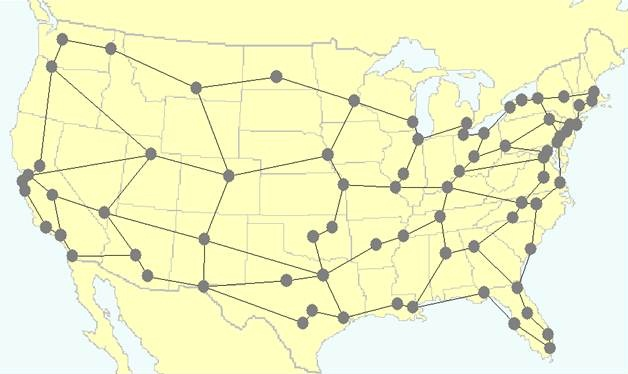
\includegraphics[width=\columnwidth]{Report//graphs/coro.jpg}}
\caption{CORONET CONUS Topology ~\cite{ref:coronus}}
\label{pruning}
\end{center}
\vskip -0.2in
\end{figure}
This topology is a real world topology between different cities in the United State of America ~\cite{ref:coronus}. It consists of 60 Nodes and 79 links. In our experiment, each link in the network has a capacity(bandwidth) of 1000 units. The VNFs are deployed on top 30\% of the nodes based on the degree of the nodes. There are a total of 20 Virtual Network Functions. Each function node, hosts 8 different types of virtual network functions. Therefore, 18 nodes each with 8 different types of virtual network functions gives a total of 144 Virtual Network Function deployments across the network. Since many virtual network functions are deployed on a single node, the processing capacity of each functional node was kept to be 1000 units. 

\subsection{Experiment Configuration}
In this section, we will discuss about the different configurations and constraints we removed or added in each experiment make the comparison fair. 

\subsubsection{Comparison on Fat-Tree}
Our first experiment was on Fat-Tree topology. The flows were generated randomly from source and destination chosen from hosts in the Fat-Tree topology. The number of virtual network functions required by a particular flow request can be up to 6. Also, for RA-RA flows with less than 2 units capacity are considered mice flows and are given high priority.  To make the comparison fair, we assume that each flow takes equal bandwidth over all the links. The capacity of each flow is assigned randomly  between 1 and 5 units. Similarly it is assumed that each flow uses the same capacity for every middlebox function and is randomly assigned between 1 and 4 units. 

\subsubsection{Comparison on CORONET CONUS}
In our second experiment on CORONET CONUS topology, the flows were generated in a different manner. The source and destination nodes could be any of the nodes in the network and are chosen randomly for a given flow. Also, setting the number of VNFs required by a flow to 6 was consuming a lot of processing power on all the platforms (CloudLab, AWS and Local Desktop). We therefore limited the number of Virtual Network Functions in a flow request to 3, thus limiting the length of each flow to 5. The bandwidth usage was assigned a value between 1 and 5 units and for the functional node, a value between 1 and 4 units similar to Fat-Tree topology.

\section{Results}
\label{sec:results}

TMA, PDA and RA-RA were run for different number of flows and for different topologies. The simulation was conducted on Fat Tree and CORONET CONUS topologies. The number of flows was varied from 100 to 1000 for PDA and RA-RA. For TMA, the upper bound for the number of flows was limited to 400 in the case of CORONET CONUS and to 300 in the case of Fat-Tree due to computation restrictions.  The number of pods in Fat Tree was set to 8. We measured the throughput for different number of flows. The number of flows vs throughput was plotted as shown in Figure ~\ref{fig:graph}. Figure ~\ref{fig:sub1} and Figure ~\ref{fig:sub3} compares the online algorithms PDA and RA-RA. We consider PDA under two settings : (1) $\epsilon = 0.5$ (2) $\epsilon = 0.75$. Figure ~\ref{fig:sub2} and ~\ref{fig:sub4} compares TMA with the upper bound.

The Upper Bound for throughput is the maximum achievable throughput across all flows. This is the ideal case that would be achieved when all the flows' SFC request is satisfied, which indicates that each flow in the group gets its desired bandwidth and CPU share. It is assumed that the upper bound is obtained in an environment without any constraints.

According to \cite{ref:paper1}, TMA achieves the maximum throughput under practical settings. This can be observed in Figure ~\ref{fig:sub2} and Figure ~\ref{fig:sub4}. For both Fat-Tree and CORONET CONUS topologies, the throughput achieved by TMA is almost equal to the Upper Bound throughput achieved under ideal conditions. However, there is a slight deviation from the upper bound when 300 flows are routed through the Fat Tree topology. This is because of the resource limitations in the network. The ideal case assumes that the network is free of such limitations.

In the case of PDA, the parameter $\epsilon$ provides a trade-off between maximizing the network throughput and meeting all the flows' QoS constraints. The smaller the value of $\epsilon$, the closer the algorithm is to the offline scenario and the better the throughput will be. We can observe this in Figure ~\ref{fig:sub1} and Figure ~\ref{fig:sub3}. For both the topologies PDA($\epsilon$=0.5) can be seen giving consistently better throughput than PDA($\epsilon$=0.75). 

We can also observe from the results in Figure ~\ref{fig:sub1} and Figure ~\ref{fig:sub3} that PDA, irrespective of the value of $\epsilon$ is performing better than RA-RA. The throughput of RA-RA drops slightly at high number of flows. We believe that because RA-RA uses much simpler constraints when routing a flows and checks limited number of paths out of all available paths, it leads to less throughout. Even though, we have not bench marked the execution time of the three algorithms, we observed that RA-RA produces the results much faster than the PDA and TMA algorithms. 

\section{Related Work}
\label{sec:relatedwork}
\cite{ref:paper2} proposes the RA-RA algorithm for resource aware routing for service function chains in SDN and NFV enabled networks. They conduct a MATLAB simulation on CORONET CONUS topology. They compare RA-RA with COATS, SP and Eigendecomposition algorithms. These algorithms use the shortest path routing to route the flows and use a greedy approach to find an optimal matching between the SFC request and network topology. It is observed that RA-RA performs the best among these algorithms. \cite{ref:paper1} compares TMA and PDA with Random, Greedy and Upper Bound algorithms. In their study TMA performs the best(close to Upper Bound) followed by PDA.

Our results show that among the online algorithms, PDA performs better than RA-RA. The performance of TMA is comparable to the ideal case where all the flows can be routed through a given network without any constraints. 
\section{Conclusion and Future Work}
\label{sec:conclusion}

In this paper, we did a comparative study of offline and online algorithms for dynamic service function chaining in SDN-Enabled Networks. We implemented a part of TMA algorithm and Primal-Dual-Update Algorithm proposed in \cite{ref:paper1} and RA-RA Algorithm proposed in \cite{ref:paper2} with the goal of maximizing the throughput. We observe that even if we consider offline scenario, the goal of achieving optimal throughput, given the constraints on resources is an NP-hard problem. Nevertheless, a convex relaxation of constrains in the practical setting can give us an optimal throughput. In the online setting, we compared the performance of PDA and RA-RA on two topologies, Fat-Tree and CORONET CONUS. We observed that PDA consistently gave better throughput than RA-RA even when the trade-off parameter, $\epsilon$, in the PDA algorithm was set to be more sensitive to meeting QoS requirements and allow less traffic through the network.

In the future, the comparison can be stretched in many directions. As discussed in the paper, for small flows we can use the offline algorithm (TFA) and for elephant flows, we can use the online (PDA) routing algorithm and compare the results. We can also conduct comparisons with various other topologies. 
Another aspect of Service function chaining is service function placement. As these service functions or network functions run on virtualized VM hardware, we can deploy the network functions anywhere in the network. Once we have deployed the network functions optimally by learning about the flows in the offline mode, we can use the offline routing algorithm and maximize the throughput. We can compare these results with our current simulation with fixed randomly distributed service functions.




{
\bibliographystyle{unsrt}
\bibliography{paper}
}
\end{document}
